\documentclass[11pt,a4paper]{article}

\usepackage[paperwidth=16cm,paperheight=23cm]{geometry}

\usepackage[utf8]{inputenc}
\usepackage{ngerman}
\usepackage{amsmath}
\usepackage{xcolor}
\definecolor{grey}{rgb}{0.9,0.9,0.9} % Colour of the box surrounding the title
% usenames allows you to use names of the default colors, the same 16 base colors as used in HTML. The dvipsnames allows you access to more colors, another 64, and svgnames allows access to about 150 colors. The initialization of "table" allows colors to be added to tables by placing the color command just before the table. If you need more colors, then you may also want to look at adding the x11names to the initialization section as well, this offers more than 300 colors, but you need to make sure your xcolor package is the most recent you can download.



\usepackage{endnotes}

\usepackage{graphicx}
\graphicspath{{Bilder/}}
\usepackage[autostyle=true,german=quotes]{csquotes}
\usepackage{enumitem}
\usepackage[T1]{fontenc}

\usepackage[onehalfspacing]{setspace}
%\renewcommand{\familydefault}{\sfdefault}

\date{}
\author{Jan Philip Wahle, Marvin Janosch, Dennis Szczepanski, Khalid Bellouch
        \and Jan-Alexander Amann}
\title{Benutzerhandbuch Autonomes Fahren}



\begin{document}

\begin{titlepage}
	\centering
	
\includegraphics[width=0.5\textwidth]{uni.png}\par\vspace{1cm}
	{\scshape\LARGE Praktikum Softwaretechnologie\par}
	\vspace{1cm}
	{\scshape\Large Gruppe 3\par}
	\vspace{1.5cm}
	\begin{center}
		
\includegraphics[width=0.35\textwidth]{icon}
	\end{center}
	{\huge\bfseries Autonomes Fahren\par}
	\vspace{2cm}
	{\Large\itshape Benutzerhandbuch\par}
	%\vfill
	%erstellt von\par
    %\textsc{Jan-Alexander Amann}

	\vfill

% Bottom of the page
	{\large \today\par}
\end{titlepage}

% Inhaltsverzeichnis anzeigen
\tableofcontents

% Kapitel soll auf naechster Seite beginnen
\newpage

\section{Installation}

\subsection{Systemanforderungen}
Damit Sie die Software ausführen können und die Simulation ausreichend schnell abläuft, benötigen sie mindestens folgende Komponenten in ihrem PC:
\begin{itemize}
\item Windows, macOS, Linux
\item 2 GHz CPU
\item 4 GB RAM
\end{itemize}

\subsection{Installationsprozess}

Entpacken Sie das Programmpaket in einen beliebigen Installationsordner.

\subsection{Erste Schritte}

Nach dem Programmstart befinden sie sich im Editor. Erstellen sie eine Strecke oder simulieren Sie eine bereits vorhandene Streckendatei.

\newpage
\section{Einführung in die Software}
Mit diesem Programm werden realitätsnahe Szenarien aus dem Straßenverkehr abstrahiert um sie dann zu simulieren. \\
Das System lernt eigenständig vorgegebene Strecken zu absolvieren und weicht dabei statischen und dynamischen Hindernissen aus.

\subsection{Map erstellen}
{
\begin{center}
	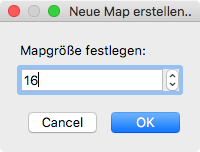
\includegraphics[width=130pt]{newMap}
\end{center}
Erstellen sie zunächst über „Datei $\rightarrow$ Neu“ in der Menüleiste oder über „
\includegraphics[height=11pt]{icon/new_map} Neue Map“ in der Schnellzugriffsleiste eine neue Karte und geben sie deren Größe an. \\
Als nächstes können Sie jedem Feld ein Streckenteil zuordnen und diverse Hindernisse auf die Felder setzen.
Überhalb der Map finden Sie Streckenteile und Hindernisse die Sie auf der Karte setzen können.\\
\begin{center}
	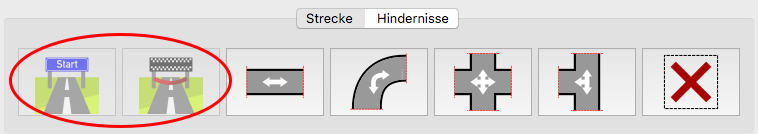
\includegraphics[width=0.9\textwidth]{s3}
\end{center}

Start- und Zielpunkt müssen gesetzt werden, bevor eine Simulation durchgeführt wird. Die erstellte Strecke kann gespeichert und dann in die Simulation geladen werden. \\
}
\subsection{Map ändern}
Öffnen sie eine bereits erstellte Map mit „Datei $\rightarrow$ Map laden“ oder mit „
\includegraphics[height=11pt]{icon/load} Map laden“ in der Schnellzugriffsleiste. Sie können diese Map nun nach ihren Wünschen anpassen. 
Anschließend können sie die Map wieder speichern.

\subsection{Map speichern}
Eine Map kann gespeichert werden indem sie in der Menü-Leiste „Datei $\rightarrow$ Map speichern“ oder in der Schnellzugriffsleiste „
\includegraphics[height=11pt]{icon/save} Map speichern“ auswählen. Geben sie einen Dateipfad an unter dem die Strecke gespeichert werden soll.
%\subsection{Fahrzeug erstellen}
%Erstellen sie ein neues Fahrzeug, indem sie in der Menü-Leiste „Datei $\rightarrow$ Neu $\rightarrow$ Fahrzeug“ auswählen. Sie müssen nun eine Mapdatei auswählen, für die das Fahrzeug erstellt werden soll. Nun geben Sie alle relevanten Fahrzeugdaten an. Anschließend wird das Fahrzeug in der Mapdatei gespeichert. Anschließend wird getestet ob das Fahrzeug die Strecke passieren kann.
\newpage
\section{Simulation}
%Simulationen können in 2D und 3D durchgeführt werden.
Die Simulation läuft nach dem Start bis das Fahrzeug den Zielpunkt erreicht hat oder eine Kollision besteht.
Des Weiteren kann die Simulation vom Benutzer pausiert oder gestoppt werden.

\subsection{Neuronales Netz erstellen / laden}
Sie können ein neues neuronales Netz erstellen 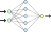
\includegraphics[height=11pt]{icon/create_Neural_network} oder ein bereits vorhandenes laden 
\includegraphics[height=11pt]{icon/load}.
\subsubsection{Neuronales Netz erstellen}
Klicken Sie auf die Schaltfläche „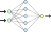
\includegraphics[height=11pt]{icon/create_Neural_network} Neuronales Netz erstellen“ und geben Sie an, wie viele Hidden Layer mit jeweils wie vielen Neuronen das Netzwerk enthalten soll. Folgen Sie den Bildschirmanweisungen.


\subsubsection{Neuronales Netz trainieren}
Zum Trainieren des neuronalen Netzes öffnen Sie den gewünschten Testkurs und klicken auf die Schaltfläche „Train Model“ oberhalb der Karte.
\begin{center}
	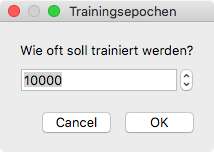
\includegraphics[width=120pt]{s5}
\end{center}
Anschließend wählen Sie aus, wie viele Runden lang das System trainieren soll und bestätigen die Eingabe.

\subsection{Simulationsmodi umschalten}
Die Simulation bietet sowohl einen Trainings-, als auch einen „autonom Fahren“-Modus.

\begin{center}
	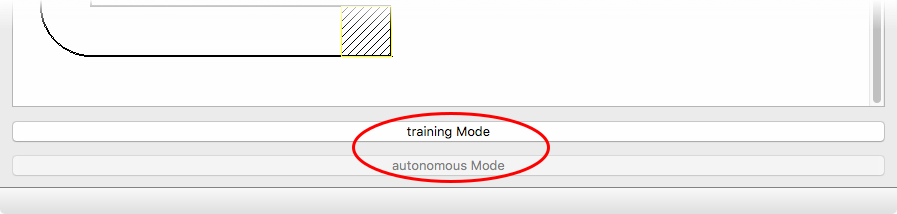
\includegraphics[width=\textwidth]{s6}
\end{center}

Diese können, wie gezeigt, am unteren Rand des Simulationsfensters umgeschaltet werden. 

\subsection{Simulation starten}
Um eine Strecke in die Simulation zu laden wählen sie in der Menüleiste „Simulation $\rightarrow$ Simulation starten“ oder in der Schnellzugriffsleiste „
\includegraphics[height=11pt]{icon/run} Simulation starten“. % und geben sie an ob die Simulation in 2D oder 3D erfolgen soll.
\subsection{Simulation stoppen oder pausieren}
Um die Simulation zu 
\includegraphics[height=11pt]{icon/pause} pausieren, 
\includegraphics[height=11pt]{icon/resume_play} fortzusetzen oder zum Stoppen klicken Sie auf die entsprechende Schaltfläche in der Simulation.
\newpage
\section{Kontakt und Support}
\textbf{Mitwirkende} \\ 
Jan Philip Wahle \\
Marvin Janosch \\
Dennis Szczepanski \\
Khalid Bellouch \\
Jan-Alexander Amann \\
\\
\textbf{Kontakt} \\ 
Bei Fragen und Problemen wenden sie sich bitte an das Entwickler-Team unter der Mail-Adresse 1521361@uni-wuppertal.de


\end{document}